% !TEX root = paper.tex
% !TEX encoding = UTF-8 Unicode

\begin{figure}
\begin{subfigure}[b]{\linewidth}
\begin{center}
\caption{Russian-English}
\label{fig:mean_adequacy_score_ru}
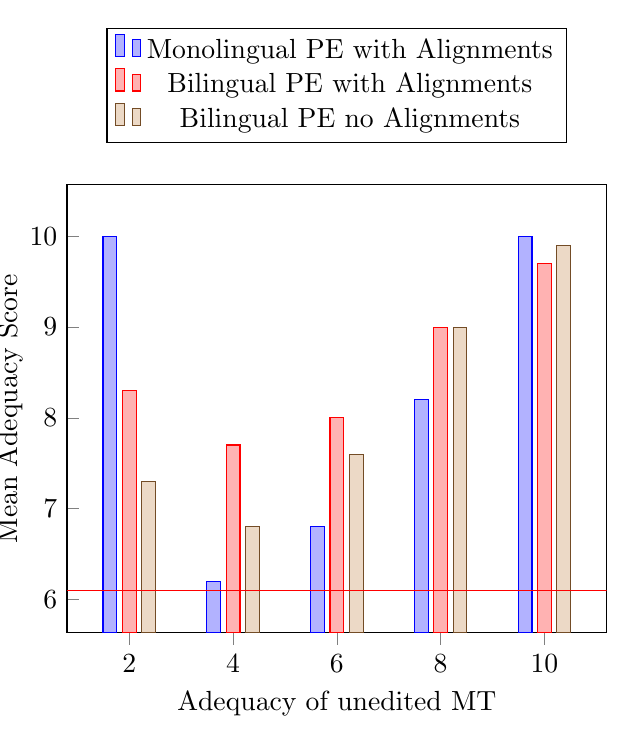
\begin{tikzpicture}[trim left={(-0.5,0)}]
\begin{axis}[
	%at={(10,0)},
	x tick label style={
		/pgf/number format/1000 sep=},
	ylabel shift={-0.15cm},
	ylabel=Mean Adequacy Score,
	enlargelimits=0.15,
	xtick pos=left,
	ytick pos=left,
	xlabel={Adequacy of unedited MT},
	%,
%	legend style={at={(0.5,-0.15)}},
%		anchor=north,legend columns=-1},
	legend style={at={(0.5,1.35)},anchor=north},
	ybar,
	bar width=5pt,
]
\addplot 
	coordinates {(2,10.0) (4,6.2)
		 (6,6.8) (8,8.2) (10,10)};

\addplot 
	coordinates {(2,8.3) (4,7.7)
		 (6,8.0) (8,9.0) (10,9.7)};

\addplot 
	coordinates {(2,7.3) (4,6.8)
		 (6,7.6) (8,9.0) (10,9.9)};

\addplot[red,sharp plot,update limits=false] 
	coordinates {(-1,6.1) (12,6.1)};

\legend{Monolingual PE with Alignments,Bilingual PE with Alignments,Bilingual PE no Alignments}
\end{axis}
\end{tikzpicture}
\end{center}
\end{subfigure}
\ \\
\begin{subfigure}[b]{\linewidth}
\begin{center}
\caption{Spanish-English}
\label{fig:mean_adequacy_score_es}
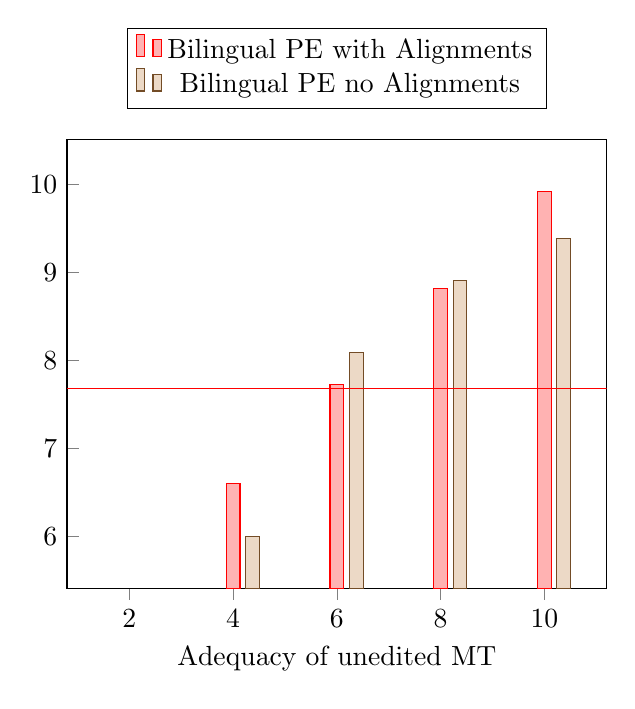
\begin{tikzpicture}[trim left={(-0.5,0)}]
\begin{axis}[
	%at={(10,0)},
	x tick label style={
		/pgf/number format/1000 sep=},
	ylabel shift={-0.15cm},
%	ylabel=Mean Adequacy Score,
	enlargelimits=0.15,
	xtick pos=left,
	ytick pos=left,
	xlabel={Adequacy of unedited MT},
	legend style={at={(0.5,1.25)},anchor=north},
	ybar,
	xmin=2,
	bar width=5pt,
]
\addplot 
	coordinates {};

\addplot coordinates {(4,6.6) (6,7.7272727272727275) (8,8.818181818181818) (10,9.923076923076923) };
\addplot coordinates {(4,6.0) (6,8.090909090909092) (8,8.909090909090908) (10,9.384615384615385) };
\addplot[red,sharp plot,update limits=false] coordinates { (-1,7.686274509803922) (12,7.686274509803922) };

\legend{Bilingual PE with Alignments,Bilingual PE no Alignments}
\end{axis}
\end{tikzpicture}
\end{center}
\end{subfigure}
\caption{Mean adequacy score, categorized by the adequacy score of the unedited MT. The red horizontal line indicates the mean adequacy score (Russian-English: 6.1; Spanish-English: 7.7) of the unedited MT.}
\label{fig:mean_adequacy_score}
\end{figure}

